\documentclass[aspectratio=169,11pt]{beamer}
\usepackage[T1]{fontenc}
\usepackage{lmodern,amsmath,amssymb,booktabs,graphicx}
\definecolor{ink}{HTML}{17324D}
\definecolor{accent}{HTML}{007C83}
\setbeamercolor{normal text}{fg=ink,bg=white}
\setbeamercolor{structure}{fg=accent}
\setbeamercolor{frametitle}{fg=ink}
\setbeamerfont{frametitle}{series=\bfseries,size=\large}
\setbeamertemplate{navigation symbols}{}
\newcommand{\deckpart}{Main talk}
\setbeamertemplate{footline}{\hbox to \paperwidth{\hfill\scriptsize ECON 847\quad Yifan and Wenhan\quad\deckpart\quad\insertframenumber\hspace{5mm}}\vskip3mm}
\setbeamersize{text margin left=8mm,text margin right=8mm}
\newcommand{\captiontext}[1]{\par\medskip{\small\raggedright #1\par}}
\hypersetup{pdftitle={Bathroom tissue: a conditional merger exercise},pdfauthor={Yifan and Wenhan}}
\begin{document}

\begin{frame}[plain]
\vspace{12mm}{\LARGE\bfseries Bathroom tissue:\\[3mm]a conditional merger exercise}\par
\vspace{8mm}{\large Scott and Kimberly-Clark under 1991--1992 conditions}\par
\vspace{9mm}Yifan and Wenhan\par ECON 847\quad November 23, 2026
\end{frame}

\begin{frame}{The merger raises prices, with a fragile supply interpretation}
\begin{itemize}\setlength\itemsep{3mm}
\item Combine Scott and Kimberly-Clark's portfolios; manufacturers reset prices.
\item Hold demand conditions, product sets and costs fixed. No merger efficiencies.
\item Across maintained scenarios: category prices rise \textbf{0.2--3.4\%}; Kimberly-Clark prices rise \textbf{1--24\%}.
\item The implied cost of Scott single rolls is often negative. That limits how we interpret the predicted increases.
\end{itemize}
\captiontext{The actual merger occurred in 1995. We simulate earlier conditions, not that transaction's remedies or efficiencies. The scenario ranges are not confidence intervals.}
\end{frame}

\begin{frame}{Scott dominates package sales; Kimberly-Clark is smaller}
\begin{columns}[T]
\column{.61\textwidth}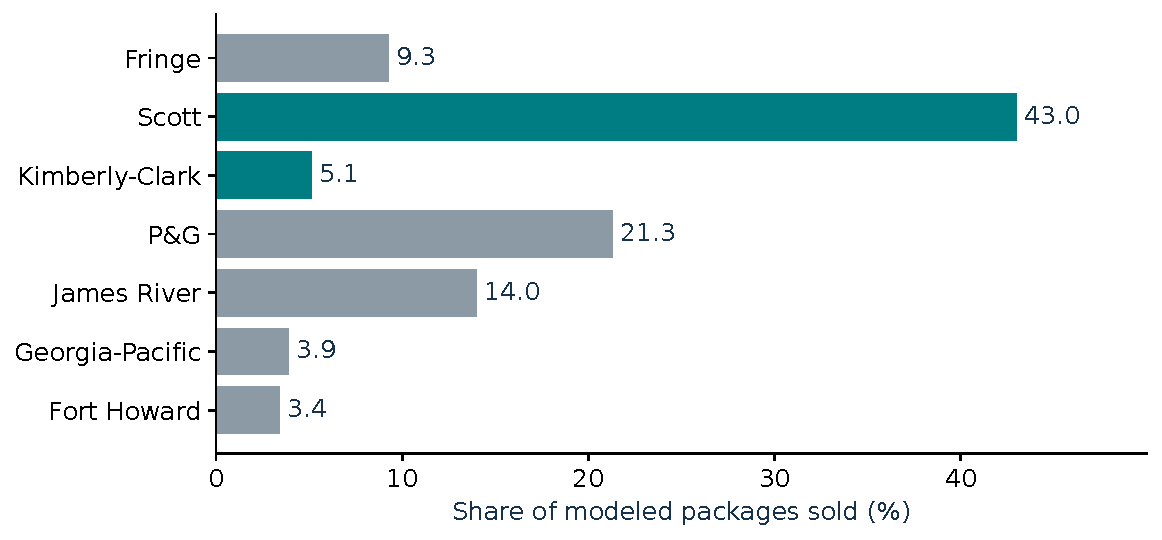
\includegraphics[width=\linewidth]{figures/manufacturers.pdf}
\column{.37\textwidth}\small
\textbf{Scott: 43\%}; ScotTissue and Cottonelle.\par\medskip
\textbf{Kimberly-Clark: 5\%}; Kleenex and Delsey. Kleenex Bath Tissue rolled out in selected regions in 1991.\par\medskip
K--C's small sales weight helps explain why its price effect can be large while the category average is modest.
\end{columns}
\captiontext{Shares of packages sold in our retail-chain sample, not national shares. Pack sizes and quality differ; private label/generics remain in demand with fixed prices.}
\end{frame}

\begin{frame}{Store-week markets retain temporary price changes}
\begin{columns}[T]
\column{.43\textwidth}
\begin{tabular}{lr}\toprule
Store-weeks & 7,996\\
Stores / UPCs & 83 / 50\\
Median UPCs per market & 32\\
Median package price & \$1.15\\
Single-roll sales volume & 37.7\%\\\bottomrule
\end{tabular}
\column{.54\textwidth}
\textbf{Store-week:} weekly temporary price cuts would be blurred by time aggregation.\par\medskip
\textbf{UPC:} retain brand, pack size and variant substitution.\par\medskip
\textbf{Share:} packages / shopping trips. Outside: no modeled package purchased.
\end{columns}
\captiontext{Positive-price/share observations and complete traffic weeks; 259,986 rows, retaining 94.31\% of broader-panel packages. Availability and units per buyer are not observed.}
\end{frame}

\begin{frame}{A typical market has many small product shares}
\centering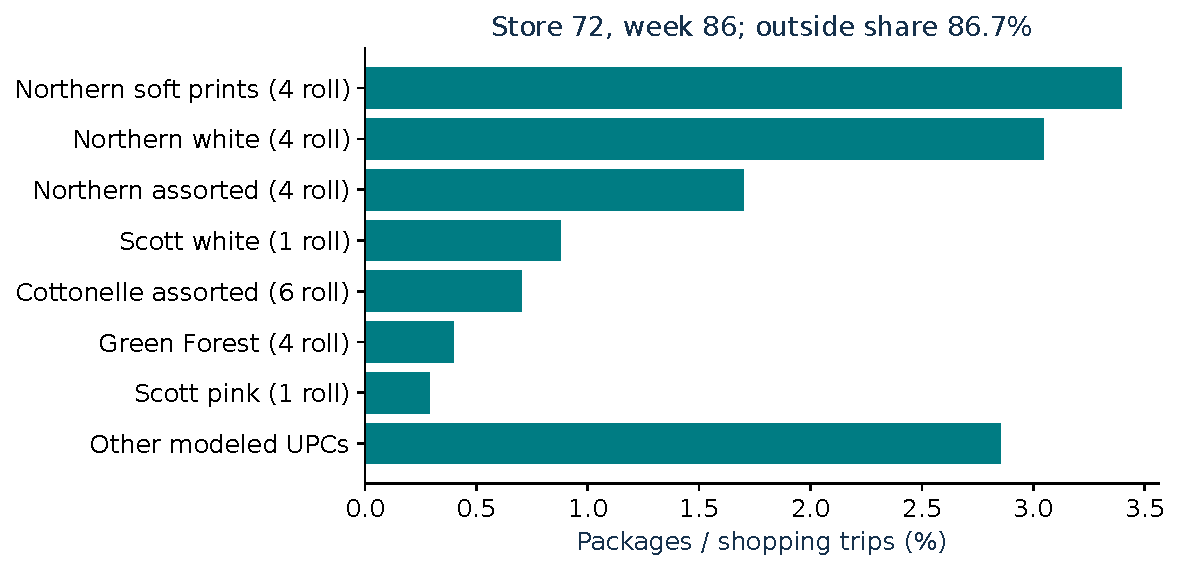
\includegraphics[height=.64\textheight]{figures/typical_market.pdf}
\captiontext{Top seven UPCs and the remaining products. Market selected near median purchase share and product count, without consulting merger predictions.}
\end{frame}

\begin{frame}{Temporary price cuts coincide with purchase spikes}
\centering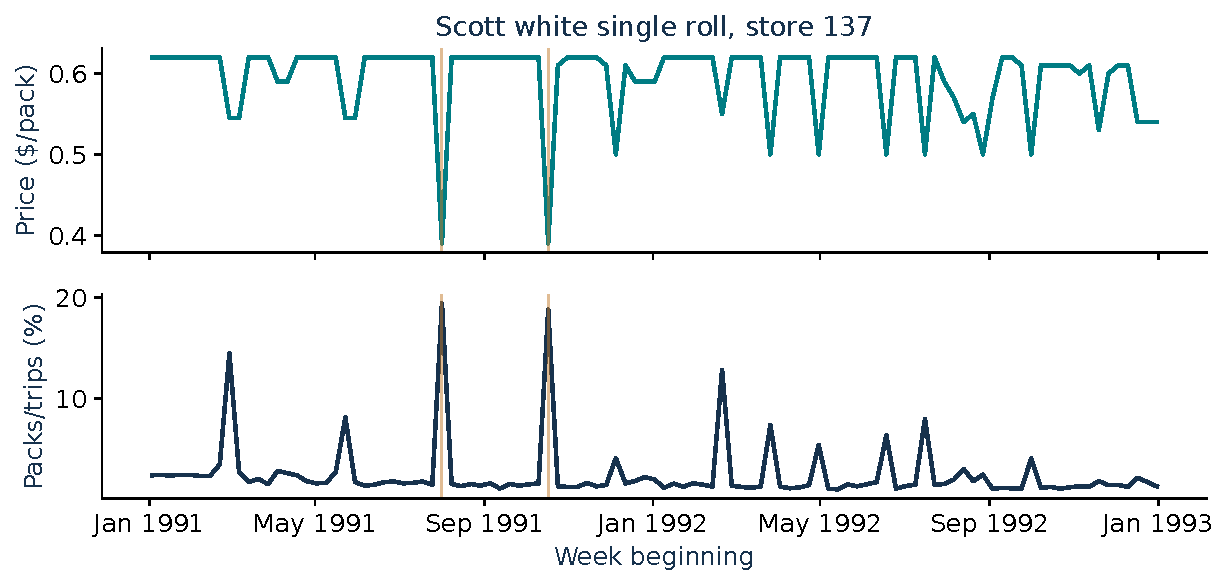
\includegraphics[height=.59\textheight]{figures/promotions.pdf}
\captiontext{Across store--UPC mean prices: 98.1\% of pooled price variance. Within a store--UPC over time: 1.9\%; these movements include sharp temporary cuts.}
\end{frame}

\begin{frame}{Demand uses price variation after fixed effects}
\[
\log\frac{s_{jt}}{s_{0t}}-\rho\log\frac{s_{jt}}{S_t}
=\alpha_{j,\mathrm{store}}+\tau_t+\beta f(p_{jt})+\gamma\,\mathrm{Deal}_{jt}+\xi_{jt}.
\]
\begin{itemize}\setlength\itemsep{2.5mm}
\item Linear or log package price; one inside nest and an outside option.
\item Absorb store--UPC and week effects, then estimate by 2SLS.
\item $\xi$ includes local demand shocks and unrecorded promotion activity: \textbf{12.5\% of packages} sell at a discount without a deal flag.
\item Calibrate $\rho\in\{0,.25,.50,.75\}$. One price instrument cannot also identify nesting. Deal is maintained exogenous.
\end{itemize}
\captiontext{Discount means more than 5\% below the store--UPC modal price. This proxy differs from the recorded deal flag; it does not prove a recording error.}
\end{frame}

\begin{frame}{Other-zone prices closely track local prices}
\small
First stage: $f(p_{jt})=\alpha^p_{j,\mathrm{store}}+\tau^p_t+\pi z_{jt}+\eta\,\mathrm{Deal}_{jt}+v_{jt}$.
\begin{center}\begin{tabular}{lrrrr}\toprule
Price / instrument & $\hat\pi$ & SE & Partial $R^2$ & Wald $\chi^2$\\\midrule
Linear / AAC & .394 & .039 & .125 & 101.4\\
Linear / other zone & 1.052 & .029 & .693 & 1315.6\\
Log / AAC & .318 & .048 & .111 & 44.6\\
Log / other zone & 1.022 & .018 & .788 & 3245.7\\\bottomrule
\end{tabular}\end{center}
\normalsize
AAC may reflect demand-related promotions. Other-zone prices may share chain-wide promotions and demand shocks. High relevance does not establish exclusion.
\captiontext{Use level instruments with linear price and log instruments with log price; each needs its own $E[\widetilde z\xi]=0$ restriction. SEs cluster by store/month. Wald is not an effective-F statistic.}
\end{frame}

\begin{frame}{Price form changes both sensitivity and pack-size elasticities}
\small
\begin{center}\begin{tabular}{lrrr}\toprule
Simple-logit demand & Price coefficient & SE & Median own elasticity\\\midrule
Linear / AAC & $-2.028$ & .319 & $-2.326$\\
Linear / other zone & $-2.689$ & .164 & $-3.084$\\
Log / AAC & $-5.388$ & .558 & $-5.376$\\
Log / other zone & $-5.184$ & .209 & $-5.173$\\\bottomrule
\end{tabular}\end{center}
\begin{center}\begin{tabular}{lrrr}\toprule
Pack size (AAC instrument) & Mean price & Linear elasticity & Log elasticity\\\midrule
One roll & \$0.51 & $-1.00$ & $-5.18$\\
Four rolls & \$1.04 & $-2.04$ & $-5.21$\\
Six or more rolls & \$2.85 & $-5.77$ & $-5.37$\\\bottomrule
\end{tabular}\end{center}
\captiontext{Top: full-sample estimates; SEs cluster by store/month, with 24 months. Bottom: package-weighted means on the same full input sample. Coefficient units differ by price form.}
\end{frame}

\begin{frame}{Portfolio markups determine implied costs}
\[
\max_{p_f}\ \sum_{j\in f}(p_j-c_j^{\mathrm{eff}})s_j(p),
\qquad c_j^{\mathrm{eff}}=p_j-\mu_j.
\]
\begin{itemize}\setlength\itemsep{3mm}
\item A manufacturer internalizes substitution among its products. Merger ownership changes these pricing incentives.
\item Main rule: fixed dollar retailer margins. Manufacturer cost is \textbf{AAC minus implied markup}; percentage margins are a backup sensitivity.
\item Hold recovered costs, utilities, traffic and products fixed; rivals reprice and fringe prices remain fixed.
\item Solve by \textbf{damped markup fixed-point iteration}; check baseline recovery, two starting prices and local optimality.
\end{itemize}
\end{frame}

\begin{frame}{Simple logit predicts modest category price increases}
\begin{center}\begin{tabular}{lrrr}\toprule
Price / instrument & Category & Scott & Kimberly-Clark\\\midrule
Linear / AAC & 0.38 & 0.55 & 2.82\\
Linear / other zone & 0.28 & 0.41 & 2.13\\
Log / AAC & 0.16 & 0.26 & 1.03\\
Log / other zone & 0.17 & 0.27 & 1.08\\\bottomrule
\end{tabular}\end{center}
\medskip
Scott's increases are modest; Kimberly-Clark's are larger. Its smaller sales weight limits its contribution to the category average.
\captiontext{Price changes in percent, weighted by baseline packages. Same 7,960 store-weeks with valid numerical solutions in every scenario; 97.08\% of baseline packages. Negative-cost cases remain included.}
\end{frame}

\begin{frame}{Stronger nesting greatly increases predicted price effects}
\centering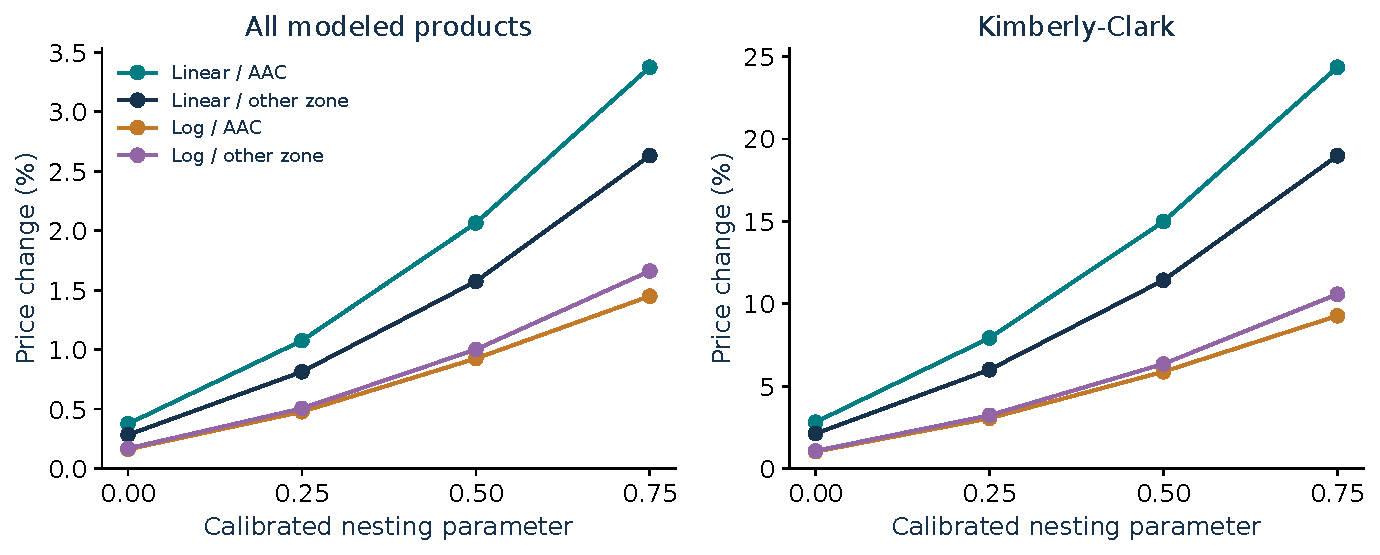
\includegraphics[width=.97\textwidth]{figures/price_sensitivity.pdf}\par
\captiontext{Nesting moves predictions most over this grid. At $\rho=.75$, median category elasticity is about $-0.48$ for linear/AAC. The largest predicted increases also occur where Scott single-roll costs fail most often.}
\end{frame}

\begin{frame}{For Scott white, the markup exceeds the wholesale proxy}
\begin{center}\small
Retail price \textbf{\$0.52}\quad AAC \textbf{\$0.48}\quad
Markup \textbf{\$0.58} at $\rho=0$, rising to \textbf{\$1.01} at $\rho=.75$\par
Implied manufacturer cost: approximately \textbf{$-\$0.10$} to \textbf{$-\$0.54$}.
\end{center}
\centering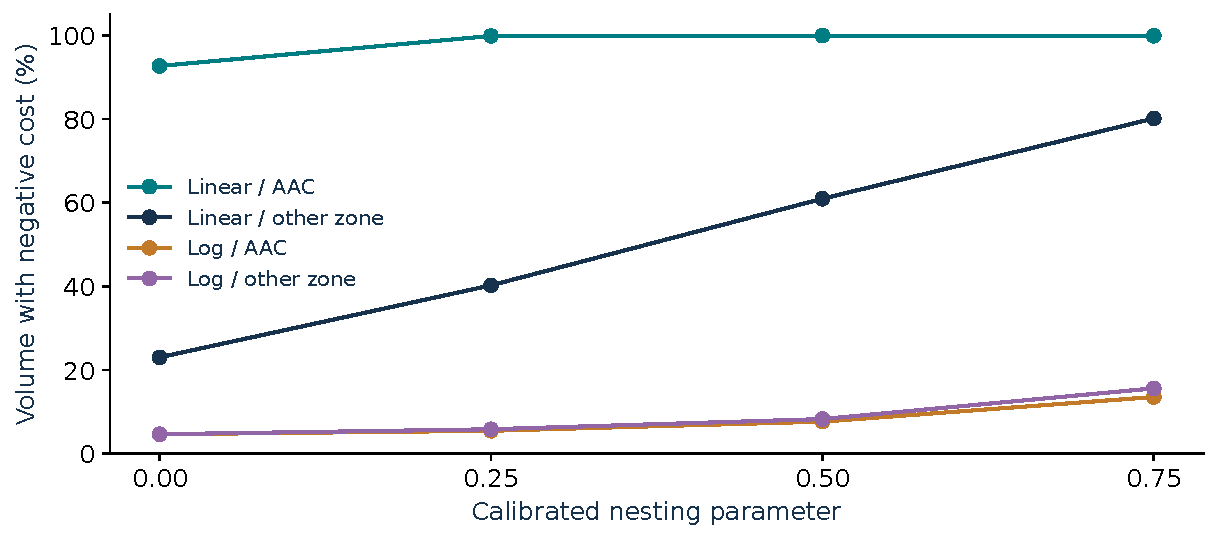
\includegraphics[height=.43\textheight]{figures/cost_failures.pdf}\par
\captiontext{Chart: share of all Scott single-roll packages with negative implied cost, full input sample, dollar margins. Example: package-weighted Scott-white means on the retained comparison markets, linear/AAC.}
\end{frame}

\begin{frame}{Cheap single rolls expose the static model's limitations}
At $\rho=0$, own-price elasticity is
\[
\varepsilon_{jj}=\begin{cases}
\beta p_j(1-s_j),&\text{linear price},\\
\beta(1-s_j),&\text{log price}.
\end{cases}
\]
\small
\textbf{Markup mechanism:} linear demand makes cheap single rolls roughly unit-elastic. For a single-product firm, $\mu_j=p_j/|\varepsilon_{jj}|$; portfolio ownership can increase the markup further.\par\medskip
\textbf{Purchase-unit problem:} store 124 records \textbf{29,209 packages against 29,213 shopping trips} in the week beginning October 17, 1991. That is a strained setting for a one-package-per-trip choice interpretation.\par\medskip
Inventory and quantity-choice behavior are plausible missing mechanisms, not identified explanations from these aggregates.
\end{frame}

\begin{frame}{The exercise shows why counterfactual assumptions matter}
\begin{itemize}\setlength\itemsep{4mm}
\item The merger raises prices under the maintained models; substitution and price form strongly affect the magnitude.
\item The specifications predicting the largest increases also imply implausible costs for a major product group.
\item Better purchase-unit measurement and credible price instruments matter more than choosing the specification with the nicest cost signs.
\end{itemize}
\medskip
\textbf{Discussion:} what new evidence would best distinguish inventory behavior, demand misspecification and retailer pricing assumptions?
\end{frame}

\appendix
\renewcommand{\deckpart}{Backup}
\begin{frame}{Retailer rules have a smaller effect in simple logit}
\small\begin{center}\begin{tabular}{lrrrr}\toprule
&\multicolumn{2}{c}{Dollar margins}&\multicolumn{2}{c}{Percentage margins}\\
&Category&K--C&Category&K--C\\\midrule
Linear / AAC & .38 & 2.82 & .37 & 3.12\\
Linear / other zone & .28 & 2.13 & .28 & 2.36\\
Log / AAC & .16 & 1.03 & .16 & 1.13\\
Log / other zone & .17 & 1.08 & .16 & 1.18\\\bottomrule
\end{tabular}\end{center}
\normalsize
Percentage margins use $q_j=1-m_j$, baseline wholesale price $q_jp_j$, and cost $q_jp_j-\mu_j$. The manufacturer/effective cost signs then agree by identity.
\captiontext{Baseline-package-weighted price changes (\%); same 7,960 markets. Comparing retailer rules does not validate AAC as manufacturer marginal cost.}
\end{frame}

\begin{frame}{Mixed-logit attempts did not resolve identification concerns}
\begin{itemize}\setlength\itemsep{3mm}
\item Eight demographic mixed-logit specifications attempted with PyBLP; six converged and two were rejected numerically.
\item Household-size or income heterogeneity; AAC or other-zone price instruments; all-pack or multipack samples.
\item Five of six saved joint tests reject. Convergence does not settle instrument validity or diagnose which maintained assumption fails.
\item We retain these attempts, but use transparent conditional logit comparisons for the classroom counterfactual.
\end{itemize}
\captiontext{This is not evidence that heterogeneity cannot help. No additional mixed-logit fits were run for the presentation. See source notes for the saved tests and specifications.}
\end{frame}

\begin{frame}{Consumer surplus falls in the linear-price scenarios}
\[
\Delta CS=\frac{\log(1+e^{L^{\mathrm{post}}/h})-\log(1+e^{L^{\mathrm{pre}}/h})}{-\beta},
\quad L=\log\sum_j e^{h\delta_j},\quad h=\frac{1}{1-\rho}.
\]
\begin{center}\begin{tabular}{lrr}\toprule
&$\rho=0$&$\rho=.75$\\\midrule
AAC & $-\$0.000423$ & $-\$0.003408$\\
Other zone & $-\$0.000319$ & $-\$0.002657$\\\bottomrule
\end{tabular}\end{center}
\captiontext{Dollars per shopping opportunity, traffic-weighted over the same retained markets; fixed dollar margins. Negative-cost cases included. Log-price dollar welfare is deferred without a specified income-compensation model. These are model outputs, not causal welfare estimates.}
\end{frame}
\end{document}
